\documentclass[12pt, a4paper]{article}

\usepackage{fancyhdr}
\usepackage[left=4cm, right=4cm, top=4cm, bottom=4cm]{geometry}
\usepackage[utf8]{inputenc}
\usepackage[table]{xcolor}
\usepackage{amsmath}
\usepackage{enumitem}
\usepackage{graphicx}
\usepackage{hyperref}
\usepackage{geometry}
\usepackage{booktabs}
\usepackage{tikz}
\usepackage{pgfplots}
\usepackage{subcaption}
\usepackage{floatrow}
\usepackage{xepersian}

\usetikzlibrary{arrows}
\newfloatcommand{capbtabbox}{table}[][\FBwidth]

\newcommand{\coursetitle}{شناسایی آماری الگو}
\newcommand{\doctitle}{تمرین چهارم}
\newcommand{\name}{محمدرضا غفرانی}
\newcommand{\studentno}{400131076}
\newcommand{\todaydate}{\today}

\settextfont{XB Kayhan}
\setlatintextfont{Times Newer Roman}

\pagestyle{fancy}
\lhead{\textbf{\doctitle}}
\chead{\name}
\rhead{\todaydate}

\begin{document}

\begin{flushleft}
    \name \\
    \studentno \\
    \todaydate
\end{flushleft}

\begin{center}
    \huge
    \textbf{\coursetitle}
    \break
    \large
    \doctitle
\end{center}

% suppress the fancy header on the first page only
\thispagestyle{plain}

\noindent

\section*{سوال یک}

\subsection*{قسمت الف}

فاصله هر نقطه تا هر یک از مراکز را می‌یابیم.

\begin{eqnarray*}
    ||x_1 - \mu_1|| = 2.47, & \hspace{.5cm} ||x_2 - \mu_1|| = 2.11, & \hspace{.5cm} ||x_3 - \mu_1|| = 1.52 \\
    ||x_4 - \mu_1|| = 1.40, & \hspace{.5cm} ||x_5 - \mu_1|| = 1.81, & \hspace{.5cm} ||x_6 - \mu_1|| = 2.66 \\
    ||x_7 - \mu_1|| = 1.56, & \hspace{.5cm} ||x_8 - \mu_1|| = 1.78, & \hspace{.5cm} ||x_9 - \mu_1|| = 1.86 \\
    & \hspace{.5cm} ||x_{10} - \mu_1|| = 2.00 &
\end{eqnarray*}

\begin{center}
    \rule{0.3\linewidth}{0.5pt}
\end{center}

\begin{eqnarray*}
    ||x_1 - \mu_2|| = 2.96, & \hspace{.5cm} ||x_2 - \mu_2|| = 1.30, & \hspace{.5cm} ||x_3 - \mu_2|| = 0.72 \\
    ||x_4 - \mu_2|| = 2.20, & \hspace{.5cm} ||x_5 - \mu_2|| = 1.07, & \hspace{.5cm} ||x_6 - \mu_2|| = 1.96 \\
    ||x_7 - \mu_2|| = 1.41, & \hspace{.5cm} ||x_8 - \mu_2|| = 2.40, & \hspace{.5cm} ||x_9 - \mu_2|| = 2.02 \\
    & \hspace{.5cm} ||x_{10} - \mu_2|| = 2.37 &
\end{eqnarray*}

\begin{center}
\rule{0.3\linewidth}{0.5pt}
\end{center}

\begin{eqnarray*}
    ||x_1 - \mu_3|| = 1.70, & \hspace{.5cm} ||x_2 - \mu_3|| = 2.22, & \hspace{.5cm} ||x_3 - \mu_3|| = 1.64 \\
    ||x_4 - \mu_3|| = 1.56, & \hspace{.5cm} ||x_5 - \mu_3|| = 2.33, & \hspace{.5cm} ||x_6 - \mu_3|| = 3.22 \\
    ||x_7 - \mu_3|| = 2.50, & \hspace{.5cm} ||x_8 - \mu_3|| = 2.66, & \hspace{.5cm} ||x_9 - \mu_3|| = 2.88 \\
    & \hspace{.5cm} ||x_{10} - \mu_3|| = 3.00 &
\end{eqnarray*}

حال هر نقطه را به نزدیک‌ترین $\mu_i$ نسبت می‌دهیم.

\begin{eqnarray*}
    \mu_1 & \Longrightarrow & \{x_4, x_8, x_9, x_{10} \} \\
    \mu_2 & \Longrightarrow & \{x_2, x_3, x_5, x_6, x_7 \} \\
    \mu_3 & \Longrightarrow & \{x_1 \}
\end{eqnarray*}

با توجه به دسته‌بندی‌های صورت گرفته مراکز جدید دسته‌ها به شکل زیر حاصل می‌شود.

\begin{eqnarray*}
    \mu_1^{(1)} & = & \frac{1}{4} (x_4 + x_8 + x_9 + x_{10}) = \begin{bmatrix}3.55& 3.25\end{bmatrix} \\
    \mu_2^{(1)} & = & \frac{1}{5} (x_2 + x_3 + x_5 + x_6 + x_7) = \begin{bmatrix}2.34 & 1.04\end{bmatrix} \\
    \mu_3^{(1)} & = & \frac{1}{1} x_1  = \begin{bmatrix}0.4& 4.5\end{bmatrix}
\end{eqnarray*}

\subsection*{قسمت ب}

مشابه قسمت قبل فاصله هر یک از داده‌ها را از مراکز به دست می‌آوریم.

\begin{eqnarray*}
    ||x_1 - \mu_1^{(1)}|| = 3.38, & \hspace{.5cm} ||x_2 - \mu_1^{(1)}|| = 3.19, & \hspace{.5cm} ||x_3 - \mu_1^{(1)}|| = 2.68 \\
    ||x_4 - \mu_1^{(1)}|| = 1.65, & \hspace{.5cm} ||x_5 - \mu_1^{(1)}|| = 2.52, & \hspace{.5cm} ||x_6 - \mu_1^{(1)}|| = 3.14 \\
    ||x_7 - \mu_1^{(1)}|| = 1.45, & \hspace{.5cm} ||x_8 - \mu_1^{(1)}|| = 0.43, & \hspace{.5cm} ||x_9 - \mu_1^{(1)}|| = 1.05 \\
    & \hspace{.5cm} ||x_{10} - \mu_1^{(1)}|| =  0.73&
\end{eqnarray*}

\begin{center}
    \rule{0.3\linewidth}{0.5pt}
\end{center}

\begin{eqnarray*}
    ||x_1 - \mu_2^{(1)}|| = 3.96, & \hspace{.5cm} ||x_2 - \mu_2^{(1)}|| = 0.87, & \hspace{.5cm} ||x_3 - \mu_2^{(1)}|| = 0.82 \\
    ||x_4 - \mu_2^{(1)}|| = 3.16, & \hspace{.5cm} ||x_5 - \mu_2^{(1)}|| = 0.07, & \hspace{.5cm} ||x_6 - \mu_2^{(1)}|| = 0.95 \\
    ||x_7 - \mu_2^{(1)}|| = 1.30, & \hspace{.5cm} ||x_8 - \mu_2^{(1)}|| = 2.94, & \hspace{.5cm} ||x_9 - \mu_2^{(1)}|| = 2.08 \\
    & \hspace{.5cm} ||x_{10} - \mu_2^{(1)}|| = 2.63 &
\end{eqnarray*}

\begin{center}
    \rule{0.3\linewidth}{0.5pt}
\end{center}

\begin{eqnarray*}
    ||x_1 - \mu_3^{(1)}|| = 0, & \hspace{.5cm} ||x_2 - \mu_3^{(1)}|| = 3.86, & \hspace{.5cm} ||x_3 - \mu_3^{(1)}|| = 3.32 \\
    ||x_4 - \mu_3^{(1)}|| = 1.82, & \hspace{.5cm} ||x_5 - \mu_3^{(1)}|| = 4.03, & \hspace{.5cm} ||x_6 - \mu_3^{(1)}|| = 4.92 \\
    ||x_7 - \mu_3^{(1)}|| = 4.03, & \hspace{.5cm} ||x_8 - \mu_3^{(1)}|| = 3.51, & \hspace{.5cm} ||x_9 - \mu_3^{(1)}|| = 4.21 \\
    & \hspace{.5cm} ||x_{10} - \mu_3^{(1)}|| = 4.12 &
\end{eqnarray*}

حال هر نقطه را به نزدیک‌ترین $\mu_i$ نسبت می‌دهیم.

\begin{eqnarray*}
    \mu_1 & \Longrightarrow & \{x_4, x_8, x_9, x_{10} \} \\
    \mu_2 & \Longrightarrow & \{x_2, x_3, x_5, x_6, x_7 \} \\
    \mu_3 & \Longrightarrow & \{x_1 \}
\end{eqnarray*}

بنابراین مراکز جدید به شکل زیر حاصل می‌شوند، با توجه به این که تغییری در نقاط هر دسته ایجاد نشده است؛ در نتیجه
مراکز دسته‌ها بدون تغییر باقی می‌ماند. بنابراین

\begin{eqnarray*}
    \mu_1^{(2)} & = & \begin{bmatrix}3.55& 3.25\end{bmatrix} \\
    \mu_2^{(2)} & = & \begin{bmatrix}2.34 & 1.04\end{bmatrix} \\
    \mu_3^{(2)} & = & \begin{bmatrix}0.4& 4.5\end{bmatrix}
\end{eqnarray*}

\subsection*{قسمت ج}

همان‌طور که در قسمت قبل دیدیم با انجام مجدد دسته‌بندی مراکز داده‌ها تغییری نکرد. بنابراین الگوریتم همگرا شده است
و در نتیجه پاسخ سوال برابر $\begin{bmatrix}0.4& 4.5\end{bmatrix}$ می‌شود.

\subsection*{قسمت د}

همان‌طور که مشاهده می‌شود با یک مرتبه اجرای الگوریتم، الگوریتم به همگرایی رسید و با انجام مجدد مراحل
دسته‌بندی در قسمت ب تغییری در دسته‌های الگوریتم مشاهده نشد.

\subsection*{قسمت ه}

خوشه‌بندی بهینه در حالتی است که داده‌های $\{-3, 0\}$ در یک خوشه و داده $8$ در خوشه دوم قرار گیرد.
اگر $\mu_1$ به طریقی انتخاب شود که داده $-3$ به خوشه آن و مرکز $\mu_2$ به صورتی
انتخاب شود که داده $8$ به خوشه آن نسبت داده شود، در این صورت خوشه‌بندی انجام شده بهینه خواهد بود.
بنابراین شروط زیر را برای $\mu_1$ و $\mu_2$ تعیین می‌کنیم.

\begin{eqnarray*}
    |-3-\mu_1| & < & |-3-\mu_2| \\
    |8-\mu_1| & > & |8-\mu_2| \\
\end{eqnarray*}

\clearpage

\subsection*{قسمت و}

اجرای الگوریتم \lr{signle-linkage} در جدول \ref{single_linkage} آورده شده است. دقت کنید که
چون به جای فاصله از شباهت در صورت سوال استفاده شده است، بنابراین به جای دو گره نزدیک
به یکدیگر، دو شبیه‌ترین گره با هم ادغام شده است.

\begin{latin}
\begin{table}[h]
    \caption{}
    \label{single_linkage}
    \begin{subtable}{0.45\linewidth}
    \caption{}
    \begin{tabular}{c|c|c|c|c|c}
              & $P_2$  & $P_3$  & $P_4$                        & $P_5$  & $P_6$  \\
        \hline
        $P_1$ & $0.52$ & $0.47$ & $0.52$                       & $0.31$ & $0.37$ \\
        \hline
        $P_2$ &        & $0.39$ & \cellcolor{purple!30} $0.53$ & $0.47$ & $0.46$ \\
        \hline
        $P_3$ &        &        & $0.28$                       & $0.40$ & $0.44$ \\
        \hline
        $P_4$ &        &        &                              & $0.50$ & $0.38$ \\
        \hline
        $P_5$ &        &        &                              &        & $0.44$ \\
    \end{tabular}
    \end{subtable}
    \hfill
    \begin{subtable}{0.45\linewidth}
    \caption{}
    \begin{tabular}{c|c|c|c|c}
        & $P_3$  & $P_5$  & $P_6$ & $(P_2, P_4)$  \\
        \hline
        $P_1$ & $0.47$ & $0.31$ & $0.37$ & \cellcolor{purple!30} $0.52$ \\
        \hline
        $P_3$ & & $0.40$ & $0.44$ & $0.39$\\
        \hline
        $P_5$ & & & $0.44$ & $0.5$ \\
        \hline
        $P_6$ & & & & $0.46$ \\
    \end{tabular}
    \end{subtable}
    \newline
    \begin{subtable}{0.45\linewidth}
        \caption{}
        \begin{tabular}{c|c|c|c}
                  & $P_5$  & $P_6$  & $((P_2, P_4), P_1)$\\
            \hline
            $P_3$ & $0.40$ & $0.44$ & $0.47$\\
            \hline
            $P_5$ &        & $0.44$ & \cellcolor{purple!30} $0.5$\\
            \hline
            $P_6$ &        &        & $0.46$\\
        \end{tabular}
    \end{subtable}
    \hfill
    \begin{subtable}{0.45\linewidth}
        \caption{}
        \begin{tabular}{c|c|c}
                  & $P_6$  & $(((P_2, P_4), P_1), P_5)$\\
            \hline
            $P_3$ & $0.44$ & \cellcolor{purple!30} $0.47$\\
            \hline
            $P_6$ &        & $0.46$\\
        \end{tabular}
    \end{subtable}
    \newline
    \begin{subtable}{0.45\linewidth}
    \caption{}
    \begin{tabular}{c|c}
              & $((((P_2, P_4), P_1), P_5), P_3)$\\
        \hline
        $P_6$ & \cellcolor{purple!30} $0.46$\\
    \end{tabular}
\end{subtable}
\end{table}
\end{latin}

\clearpage

\subsection*{قسمت ز}

اجرای الگوریتم \lr{compelte-linkage} در جدول \ref{compelete_linkage} آورده شده است. دقت کنید که
چون به جای فاصله از شباهت در صورت سوال استفاده شده است، بنابراین به جای دو گره نزدیک
به یکدیگر، دو شبیه‌ترین گره با هم ادغام شده است.

\begin{latin}
    \begin{table}[h]
        \caption{}
        \label{compelete_linkage}
        \begin{subtable}{0.45\linewidth}
            \caption{}
            \begin{tabular}{c|c|c|c|c|c}
                & $P_2$  & $P_3$  & $P_4$                        & $P_5$  & $P_6$  \\
                \hline
                $P_1$ & $0.52$ & $0.47$ & $0.52$                       & $0.31$ & $0.37$ \\
                \hline
                $P_2$ &        & $0.39$ & \cellcolor{purple!30} $0.53$ & $0.47$ & $0.46$ \\
                \hline
                $P_3$ &        &        & $0.28$                       & $0.40$ & $0.44$ \\
                \hline
                $P_4$ &        &        &                              & $0.50$ & $0.38$ \\
                \hline
                $P_5$ &        &        &                              &        & $0.44$ \\
            \end{tabular}
        \end{subtable}
        \hfill
        \begin{subtable}{0.45\linewidth}
            \caption{}
            \begin{tabular}{c|c|c|c|c}
                & $P_3$  & $P_5$  & $P_6$  & $(P_2, P_4)$ \\
                \hline
                $P_1$ & $0.47$ & $0.31$ & $0.37$ & \cellcolor{purple!30} $0.52$ \\
                \hline
                $P_3$ &        & $0.40$ & $0.44$ & $0.28$ \\
                \hline
                $P_5$ &        &        & $0.44$ & $0.47$ \\
                \hline
                $P_6$ &        &        &        & $0.38$ \\
            \end{tabular}
        \end{subtable}
        \newline
        \begin{subtable}{0.45\linewidth}
            \caption{}
            \begin{tabular}{c|c|c|c}
                & $P_5$  & $P_6$                        & $((P_2, P_4), P_1)$ \\
                \hline
                $P_3$ & $0.40$ & \cellcolor{purple!30} $0.44$ & $0.28$              \\
                \hline
                $P_5$ &        & $0.44$                       & $0.31$              \\
                \hline
                $P_6$ &        &                              & $0.37$              \\
            \end{tabular}
        \end{subtable}
        \hfill
        \begin{subtable}{0.45\linewidth}
            \caption{}
            \begin{tabular}{c|c|c}
                & $((P_2, P_4), P_1)$ & $(P_3, P_6)$ \\
                \hline
                $P_5$ & $0.31$ & \cellcolor{purple!30}$0.40$\\
                \hline
                $((P_2, P_4), P_1)$ & & $0.28$\\
            \end{tabular}
        \end{subtable}
        \newline
        \begin{subtable}{0.45\linewidth}
            \caption{}
            \begin{tabular}{c|c}
                & $((P_2, P_4), P_1)$ \\
                \hline
                $((P_3, P_6), P_5)$ & \cellcolor{purple!30} $0.28$ \\
            \end{tabular}
        \end{subtable}
    \end{table}
\end{latin}

\clearpage
\subsection*{قسمت ح}

اجرای الگوریتم \lr{average-linkage} در جدول \ref{average_linkage} آورده شده است.

\begin{latin}
    \begin{table}[h]
        \caption{}
        \label{average_linkage}
        \begin{subtable}{0.45\linewidth}
            \caption{}
            \begin{tabular}{c|c|c|c|c|c}
                      & $P_2$  & $P_3$  & $P_4$                        & $P_5$  & $P_6$  \\
                \hline
                $P_1$ & $0.52$ & $0.47$ & $0.52$                       & $0.31$ & $0.37$ \\
                \hline
                $P_2$ &        & $0.39$ & \cellcolor{purple!30} $0.53$ & $0.47$ & $0.46$ \\
                \hline
                $P_3$ &        &        & $0.28$                       & $0.40$ & $0.44$ \\
                \hline
                $P_4$ &        &        &                              & $0.50$ & $0.38$ \\
                \hline
                $P_5$ &        &        &                              &        & $0.44$ \\
            \end{tabular}
        \end{subtable}
        \hfill
        \begin{subtable}{0.45\linewidth}
            \caption{}
            \begin{tabular}{c|c|c|c|c}
                      & $P_3$  & $P_5$  & $P_6$  & $(P_2, P_4)$                 \\
                \hline
                $P_1$ & $0.47$ & $0.31$ & $0.37$ & \cellcolor{purple!30} $0.52$ \\
                \hline
                $P_3$ &        & $0.40$ & $0.44$ & $0.335$                      \\
                \hline
                $P_5$ &        &        & $0.44$ & $0.485$                      \\
                \hline
                $P_6$ &        &        &        & $0.42$                       \\
            \end{tabular}
        \end{subtable}
        \newline
        \begin{subtable}{0.45\linewidth}
            \caption{}
            \begin{tabular}{c|c|c|c}
                      & $P_5$  & $P_6$  & $((P_2, P_4), P_1)$         \\
                \hline
                $P_3$ & $0.40$ & \cellcolor{purple!30}$0.44$ & $0.38$                      \\
                \hline
                $P_5$ &        & $0.44$ & $0.426$                     \\
                \hline
                $P_6$ &        &        & $0.403$                     \\
            \end{tabular}
        \end{subtable}
        \hfill
        \begin{subtable}{0.45\linewidth}
            \caption{}
            \begin{tabular}{c|c|c}
                                    & $((P_2, P_4), P_1)$ & $(P_3, P_6)$ \\
                \hline
                $P_5$               & \cellcolor{purple!30}$0.426$             & $0.42$      \\
                \hline
                $((P_2, P_4), P_1)$ &                     & $0.391$
            \end{tabular}
        \end{subtable}
        \newline
        \begin{subtable}{0.45\linewidth}
            \caption{}
            \begin{tabular}{c|c}
                                           & $(P_3, P_6)$ \\
                \hline
                $(((P_2, P_4), P_1), P_5)$ & \cellcolor{purple!30}$0.398$
            \end{tabular}
        \end{subtable}
    \end{table}
\end{latin}

\clearpage
\thispagestyle{fancy}


\section*{سوال دوم}

\subsection*{قسمت الف}

دقت الگوریتم خوشه‌بندی برابر $0.8541$ است. لازم به ذکر است که از آن‌جا که
\lr{kMeans} یک الگوریتم خوشه‌بندی است، بنابراین ممکن است برچسب در نظر گرفته شده
برای خوشه‌ها با برچسبی که ما انتظار داریم متفاوت باشد، در این حالت دقت خوشه‌بندی
\lr{kMeans} باید با تغییر برچسب‌ها صورت گیرد.

\subsection*{قسمت ب}

دقت الگوریتم همواره برابر $0.8541$ می‌شود. خاطر نشان می‌سازد که برچسب برگردانده
شده توسط خوشه‌بندی \lr{kMeans} ممکن است با برچسب مورد انتظار ما متفاوت باشد
و در نتیجه در بعضی از موارد باید این برچسب‌ها تغییر کنند.

با توجه به آن که دقت الگوریتم همواره ثابت باقی مانده است، نتیجه گرفته می‌شود
که توزیع این داده‌ها در فضای چند بعدی به طریقی است که الگوریتم \lr{kMeans}
در مینیمم محلی‌گیر نمی‌کند و همواره به بهترین نتیجه می‌رسد.

\subsection*{قسمت ج}

در این حالت نیز دقت الگوریتم خوشه‌بندی برابر $0.8541$ می‌شود.

\subsection*{قسمت د}

در این حالت نیز دقت الگوریتم برابر $0.8541$ می‌شود.

\subsection*{قسمت ه}

الگوریتم \lr{kMeans} فرض می‌کند داده‌ها دارای توزیع‌های فشرده باشند. با توجه به آن
که این الگوریتم توانسته است روی داده‌ها به نتایج خوبی دست پیدا کند، بنابراین
می‌توان تا اظهار کرد که توزیع دسته‌ها حالت فشرده داشته است. در این حالت
می‌توان از الگوریتم \lr{single linkage} نیز برای خوشه‌بندی استفاده کرد.
این الگوریتم با توجه به آن که اتصال داده‌ها به یکدیگر را در نظر می‌گیرد،
ممکن است به نتایج بهتری دست پیدا کند.

با فرض وجود برچسب برای داده‌ها می‌توان از الگوریتم‌های دسته‌بندی نظیر
\lr{Bayes} و \lr{kNN} نیز برای دسته‌بندی استفاده کرد. استفاده از این الگوریتم‌ها
با توجه به این که معمولا به دقت بیشتری نسبت به روش‌های بدون نظارت
می‌رسند، منطقی بوده و ممکن است به دقت بهتری نسبت به روش \lr{kMeans} برسد.

\clearpage
\thispagestyle{fancy}

\section*{سوال سوم}

\subsection*{قسمت الف}

نتایج به شکل زیر حاصل می‌شود. (شکل \ref{kmeans_rand_mat})

\begin{figure}[h]
    \centering
    \begin{subfigure}{.45\linewidth}
        \includegraphics[width=\linewidth]{images/q3/a/2.png}
    \end{subfigure}
    \hfill
    \begin{subfigure}{.45\linewidth}
        \includegraphics[width=\linewidth]{images/q3/a/3.png}
    \end{subfigure}
    \newline
    \begin{subfigure}{.45\linewidth}
        \includegraphics[width=\linewidth]{images/q3/a/5.png}
    \end{subfigure}
    \hfill
    \begin{subfigure}{.45\linewidth}
        \includegraphics[width=\linewidth]{images/q3/a/10.png}
    \end{subfigure}
    \caption{نتایج دسته‌بندی دادگان \lr{rand.mat} با استفاده از الگوریتم \lr{kMeans}}
    \label{kmeans_rand_mat}
\end{figure}

\subsection*{قسمت ب}

در الگوریتم \lr{elbow} ابتدا خطای \lr{SSE} به ازای مقادیر مختلف $k$ پیدا می‌شود. سپس نمودار خطای
\lr{SSE} به ازای مقادیر مختلف $k$ رسم شده و $k$ای که به ازای آن نمودار \lr{SSE} تقریبا افقی می‌شود را
را یافته و همان را به عنوان تعداد خوشه‌های الگوریتم در نظر می‌گیرند. شکل \ref{elbow} نمودار \lr{SSE} به ازای
$k$های مختلف را برای این سوال نشان می‌دهد. همان‌طور که مشاهده می‌شود، به ازای $k=8$ نمودار تقریبا افقی می‌شود.
بنابراین روش \lr{elbow} تعداد خوشه‌های داده‌ها را $8$ پیش‌بینی می‌کند.

\newpage

\begin{figure}[t]
    \centering
    \includegraphics[scale=0.5]{images/q3/b/elbow.png}
    \caption{نمودار \lr{Elbow}}
    \label{elbow}
\end{figure}

\subsection*{قسمت ج}

نتایج به شکل زیر حاصل می‌شود. (شکل \ref{kmedoid_rand_mat})
با دقت در نتایج حاصل شده و مقایسه آن‌ها با نتایج حاصل شده در قسمت الف، مشاهده می‌شود که
هر دو الگوریتم به ازای $k=2$ و $k=3$ عملکرد یکسانی داشته‌اند، اما عملکرد روش \lr{kMdeoids}
به ازای $k$های بالاتر نسبت به \lr{kMeans} بهتر بوده و به ازای $k=5$ و $k=10$ توانسته است
یکی از دسته‌ها را به طور کامل شناسایی کند.

\begin{figure}[h]
    \centering
    \begin{subfigure}{.45\linewidth}
        \includegraphics[width=\linewidth]{images/q3/c/2.png}
    \end{subfigure}
    \hfill
    \begin{subfigure}{.45\linewidth}
        \includegraphics[width=\linewidth]{images/q3/c/3.png}
    \end{subfigure}
    \newline
    \begin{subfigure}{.45\linewidth}
        \includegraphics[width=\linewidth]{images/q3/c/5.png}
    \end{subfigure}
    \hfill
    \begin{subfigure}{.45\linewidth}
        \includegraphics[width=\linewidth]{images/q3/c/10.png}
    \end{subfigure}
    \caption{نتایج دسته‌بندی دادگان \lr{rand.mat} با استفاده از الگوریتم \lr{kMedoid}}
    \label{kmedoid_rand_mat}
\end{figure}

\clearpage

\subsection*{قسمت د}

نتایج به صورت شکل \ref{hierarchical_clustering} حاصل می‌شود. همان‌طور که مشاهده می‌شود
داده‌ها به دودویی با هم ادغام شده‌اند. این ادغام‌ها تا جایی پیش رفته است که به یک دسته
برسیم، بنابراین می‌توان با این روش‌ها داده‌ها را به دو دسته تقسیم کرد. همچنین
همان‌طور که در شکل‌ها دیده می‌شود استفاده از معیار‌های فاصله مختلف و نوع روش ادغام خوشه‌ها
در نتایج حاصل شده تاثیرگذار بوده است.

\begin{figure}[h]
    \begin{subfigure}{0.45\linewidth}
        \includegraphics[width=\linewidth]{images/q3/d/single_euclidean.png}
    \end{subfigure}
    \hfill
    \begin{subfigure}{0.45\linewidth}
        \includegraphics[width=\linewidth]{images/q3/d/single_correlation.png}
    \end{subfigure}
    \newline
    \begin{subfigure}{0.45\linewidth}
        \includegraphics[width=\linewidth]{images/q3/d/complete_euclidean.png}
    \end{subfigure}
    \hfill
    \begin{subfigure}{0.45\linewidth}
        \includegraphics[width=\linewidth]{images/q3/d/complete_correlation.png}
    \end{subfigure}
    \caption{انجام دسته‌بندی سلسله‌مراتبی با معیار‌های فاصله مختلف}
    \label{hierarchical_clustering}
\end{figure}

\subsection*{قسمت ه}

برای این کار می‌توانیم از الگوریتم‌های \lr{PCA} و \lr{Fisher} کمک بگیریم. اگر از الگوریتم
\lr{Fisher} کمک بگیریم، این الگوریتم بهترین جهتی که برای دسته‌بندی داده‌ها در فضای یک بعدی می‌توان انجام داد را
به دست می‌دهد. با بررسی وزنی که این الگوریتم برای ژن‌های مختلف در نظر می‌گیرد می‌توانیم روی تاثیرگذارترین
ژن‌ها نظر دهیم.

الگوریتم \lr{PCA} نیز مشابه الگوریتم \lr{Fisher} عمل می‌کند با این تفاوت که این الگوریتم دقیقا یک جهت را
نمی‌دهد بلکه بردار‌های مختلفی را معرفی می‌کند که با تصویر بردار‌های اولیه بر روی آن‌ها می‌توان ابعاد داده‌ها
را کاهش داد. مشابه روش \lr{Fisher}، با بررسی وزن‌های در نظر گرفته شده در بردار‌های \lr{PCA} می‌توان به
ژن‌های مهم برای دسته‌بندی پی برد.

\subsection*{قسمت و}

نتایج به صورت زیر حاصل می‌شود. الگوریتم \lr{single-linkage} مطابق انتظار، بهترین عملکرد را داشته است
و توانسته است تمامی داده‌ها را به درستی دسته‌بندی کند. اما عملکرد دو الگوریتم دیگر مشابه یکدیگر است.
چرا که این روش‌ها سعی کرده‌اند داده‌ها را از وسط صفحه به دو دسته تقسیم کنند که در نتیجه نتوانسته‌اند عملکرد خوبی
داشته باشند.

\begin{latin}
\begin{table}[h]
    \centering
    \begin{tabular}{l|c|c|c}
        & Purity & NMI \\
        \toprule
        kMeans & $0.593$ & $0.025$ \\
        single-linkage & $1$ & $1$ \\
        complete-linkage & $0.604$ & $0.036$ \\
    \end{tabular}
\end{table}
\end{latin}


\clearpage
\thispagestyle{fancy}

\section*{سوال چهارم}

\subsection*{قسمت الف}

بردار ويژه متناظر ۲۰ مقدار ویژه بزرگ در شکل \ref{q4-eigenvectors} دیده می‌شود.

\begin{figure}[h]
    \centering
    \includegraphics[width=0.7\linewidth]{images/q4/a/eigenvectors.png}
    \caption{بردار‌های ویژه متناظر ۲۰ مقدار ویژه بزرگ}
    \label{q4-eigenvectors}
\end{figure}

شکل داده‌ها پس از تصویر کردن آن‌ها بر روی بزرگترین مولفه در شکل
\ref{pca_1d_projection}، با تصویر کردن بر روی دو بزرگترین بردار‌های ویژه
در شکل \ref{pca_2d_projection} و بر روی سه بزرگترین بردار‌های ویژه
شکل \ref{pca_3d_projection} دیده می‌شود.

\begin{figure}[h]
    \centering
    \includegraphics[width=0.7\linewidth]{images/q4/a/projection_to_1d.png}
    \caption{تصویر داده‌ها بر روی بزرگترین مولفه با استفاده از روش \lr{PCA}}
    \label{pca_1d_projection}
\end{figure}

\begin{figure}[h]
    \centering
    \includegraphics[width=0.7\linewidth]{images/q4/a/projection_to_2d.png}
    \caption{تصویر داده‌ها بر روی دو بزرگترین مولفه با استفاده از روش \lr{PCA}}
    \label{pca_2d_projection}
\end{figure}

\begin{figure}[h]
    \centering
    \begin{subfigure}{0.3\linewidth}
        \centering
        \includegraphics[width=\linewidth]{images/q4/a/projection_to_3d_with_angle0.png}
    \end{subfigure}
    \hfill
    \begin{subfigure}{0.3\linewidth}
        \centering
        \includegraphics[width=\linewidth]{images/q4/a/projection_to_3d_with_angle60.png}
    \end{subfigure}
    \hfill
    \begin{subfigure}{0.3\linewidth}
        \centering
        \includegraphics[width=\linewidth]{images/q4/a/projection_to_3d_with_angle120.png}
    \end{subfigure}
    \newline
    \begin{subfigure}{0.3\linewidth}
        \centering
        \includegraphics[width=\linewidth]{images/q4/a/projection_to_3d_with_angle180.png}
    \end{subfigure}
    \hfill
    \begin{subfigure}{0.3\linewidth}
        \centering
        \includegraphics[width=\linewidth]{images/q4/a/projection_to_3d_with_angle240.png}
    \end{subfigure}
    \hfill
    \begin{subfigure}{0.3\linewidth}
        \centering
        \includegraphics[width=\linewidth]{images/q4/a/projection_to_3d_with_angle300.png}
    \end{subfigure}
    \caption{تصویر داده‌ها بر روی سه بزرگترین مولفه با استفاده از روش \lr{PCA}}
    \label{pca_3d_projection}
\end{figure}
\clearpage

\subsection*{قسمت ب}

تصویر داده‌ها بر روی فضای یک بعد و دو بعدی با استفاده از روش \lr{LDA} در
به ترتیب در شکل‌های \ref{lda_projection_1d}
و \ref{lda_projection_2d} مشاهده می‌شود.

\begin{figure}[h]
    \centering
    \includegraphics[width=0.7\linewidth]{images/q4/b/projection_to_1d.png}
    \caption{تصویر داده‌ها به فضای یک بعدی با استفاده از روش \lr{LDA}}
    \label{lda_projection_1d}
\end{figure}

\begin{figure}[h]
    \centering
    \includegraphics[width=0.7\linewidth]{images/q4/b/projection_to_2d.png}
    \caption{تصویر داده‌ها به فضای دو بعدی با استفاده از روش \lr{LDA}}
    \label{lda_projection_2d}
\end{figure}
\clearpage

\subsection*{قسمت ج}

نتایج اجرای الگوریتم \lr{K-Means} با \lr{K}های متفاوت در شکل \ref{q4kmeans}
دیده می‌شود. در نگاه اول مشخص است که با افزایش مقدار \lr{K} و
نزدیک شدن این مقدار به تعداد واقعی دسته‌های موجود، الگوریتم خوشه‌بندی
منطقی‌تری را ارائه داده است. اما در کل این الگوریتم نتوانسته است
داده‌ها را به خوبی خوشه‌بندی کند. الگوریتم \lr{K-Means} سعی می‌کند هر خوشه تا جای
ممکن شکل جمع‌وجور داشته باشد. بنابراین برای داده‌هایی که به
شکل دایره‌ای و جمع‌وجور قرار گرفته‌اند تقریبا توانسته است به
خوبی عمل کند. اما برای داده‌هایی که دارای توزیع مستطیلی شکل بوده‌اند نتوانسته است
به خوبی عمل کند.

\begin{figure}[h]
    \begin{subfigure}{0.32\linewidth}
        \includegraphics[width=\linewidth]{images/q4/c/3.png}
    \end{subfigure}
    \hfill
    \begin{subfigure}{0.32\linewidth}
        \includegraphics[width=\linewidth]{images/q4/c/7.png}
    \end{subfigure}
    \hfill
    \begin{subfigure}{0.32\linewidth}
        \includegraphics[width=\linewidth]{images/q4/c/10.png}
    \end{subfigure}
    \caption{نتایج اجرای الگوریتم \lr{K-Means} با \lr{K}های مختلف}
    \label{q4kmeans}
\end{figure}

\subsection*{قسمت د} % TODO: May Need a Better Explanation.

در این حالت خوشه‌بندی و مراکز هر خوشه مطابق شکل
\ref{q4kmeans_initial_centers_known} حاصل می‌شود.
با مقایسه خوشه‌بندی حاصل شده در این قسمت با خوشه‌بندی انجام شده در قسمت قبل
تفاوتی دیده نمی‌شود.

\begin{figure}[h]
    \begin{subfigure}{0.32\linewidth}
        \includegraphics[width=\linewidth]{images/q4/d/3.png}
    \end{subfigure}
    \hfill
    \begin{subfigure}{0.32\linewidth}
        \includegraphics[width=\linewidth]{images/q4/d/7.png}
    \end{subfigure}
    \hfill
    \begin{subfigure}{0.32\linewidth}
        \includegraphics[width=\linewidth]{images/q4/d/10.png}
    \end{subfigure}
    \caption{نتایج اجرای الگوریتم \lr{K-Means}
    با \lr{K}های مختلف و مقداردهی مراکز اولیه}
    \label{q4kmeans_initial_centers_known}
\end{figure}

\clearpage

\subsection*{قسمت ه}

برای انجام این کار از راهکار ارائه توسط وبسایت‌های زیر کمک کمک گرفته‌ایم.
خلاصه مطلب بیان شده توسط این دو وبسایت این است که برای محاسبه واریانسی که
الگوریتم \lr{PCA} در داده‌ها حفظ می‌کند باید مجموع مقادیر ویژه متناظر $n$
بردار ویژه انتخاب شده را بر مجموع همه مقادیر ویژه تقسیم کنیم.

\begin{itemize}
    \item \href{https://stats.stackexchange.com/questions/22569/pca-and-proportion-of-variance-explained}{منبع ۱}
    \item \href{https://www.mikulskibartosz.name/pca-how-to-choose-the-number-of-components/}{منبع ۲}
\end{itemize}

با انجام روش پیشنهاد شده در منابعی که بیان شد، به این نتیجه می‌رسیم با حفظ
$271$ مولفه مهم می‌توانیم $0.95$ واریانس را حذف کنیم. در ادامه در شکل
\ref{origin_and_reconstructed_image} تصاویر بازسازی شده با استفاده از
این مولفه‌ها به همراه تصاویر اصلی آورده شده است. همان‌طور که مشاهده می‌شود،
تصاویر بازسازی شده تقریبا قابل تفکیک از تصاویر اصلی نیستند و تنها تفاوت آن‌ها
در این است که در تصاویر باز‌سازی شده تعدادی نقاط سیاه‌رنگ که نویز به نظر
می‌رسند مشاهده می‌شوند.

\begin{figure}[h]
    \centering
    \includegraphics[width=0.5\linewidth]{images/q4/e/origin_and_reconstructed.png}
    \caption{تفاوت تصویر اصلی با تصویر تولید شده با استفاده از ۲۷۱ مولفه مهم}
    \label{origin_and_reconstructed_image}
\end{figure}

\subsection*{قسمت و}

در این قسمت ابتدا تصویر داده‌ها را در فضای ۲۷۱ بعدی (که در قسمت قبلی یافته بودیم)
یافته و سپس الگوریتم \lr{K-Means} با مقدار $k=10$ بر روی داده‌ها انجام می‌دهیم.
در شکل \ref{samples_for_each_cluster} نمایش ۱۰ نمونه از هر خوشه آورده شده است.

بعضی از خوشه‌ها نظیر ۱، ۳، ۴ و ۷ به نظر می‌رسد که از خلوص بالایی برخوردار باشند،
چرا که تقریبا تمامی اعضای هر خوشه شبیه هم هستند. اما الگوریتم
نتوانسته است در باقی خوشه‌ها اشیا را به خوبی از هم تمیز دهد. برای مثال شی
«ابر» و «میز» هر دو در خوشه ۶ قرار دارند و یا اشیاء «عینک» و «قیچی» هر دو در
خوشه شماره ۸ قرار گرفته‌اند. با این حال الگوریتم اشیایی که از نظر بصری
یکسان بوده‌اند را در یک خوشه قرار داده است. برای مثال در خوشه ۹ اشیایی قرار
گرفته‌اند که دارای شکلی با خطوط زیگزاگی فراوان بوده‌اند.

\begin{figure}[h]
    \centering
    \includegraphics[width=0.85\linewidth]{images/q4/f/samples.png}
    \caption{نمونه‌هایی برای هر خوشه پس از انجام الگوریتم \lr{K-Means}}
    \label{samples_for_each_cluster}
\end{figure}

\clearpage

\subsection*{قسمت ز}

نتایج در شکل \ref{distribution_in_clusters} قابل مشاهده است. بخشی از نتایج
حاصل شده در این قسمت مورد انتظار بود اما بخشی دیگر از نتایج نه. مطابق انتظار
خوشه‌های ۳، ۴ و ۷ تقریبا خالص هستند، اما خوشه ۱ که در قسمت قبلی به عنوان خالص
معرفی شد، در این قسمت مشخص می‌شود که خالص نیست. در عوض در این قسمت مشخص
است که خوشه ۸ یک خوشه خالص است.

الگوریتم به جز خوشه‌های ۲، ۵ و ۶ در باقی خوشه‌ها عملکرد قابل قبولی را به نمایش
می‌گذارد. با بررسی دقیق‌تر این خوشه‌ها متوجه می‌شویم که در همه این خوشه‌ها
دسته‌های ۰ و ۴ دارای درصد نسبتا بالا و برابر هستند که باعث شده است این خوشه‌ها
قابل قبول نباشند. از آن جا که دسته‌های ۰ و ۴ به ترتیب متناظر «ابر» و «میز»
هستند به نظر می‌رسد که عدم توانایی تفکیک این دو کلاس از هم منطقی باشد. چرا که
این دو شی دارای شکل نزدیک به هم است.

\begin{figure}[h]
    \begin{subfigure}{0.3\linewidth}
        \centering
        \includegraphics[scale=0.15]{images/q4/g/cluster0.png}
    \end{subfigure}
    \hfill
    \begin{subfigure}{0.3\linewidth}
        \centering
        \includegraphics[scale=0.15]{images/q4/g/cluster1.png}
    \end{subfigure}
    \hfill
    \begin{subfigure}{0.3\linewidth}
        \centering
        \includegraphics[scale=0.15]{images/q4/g/cluster2.png}
    \end{subfigure}
    \newline
    \begin{subfigure}{0.3\linewidth}
        \centering
        \includegraphics[scale=0.15]{images/q4/g/cluster3.png}
    \end{subfigure}
    \hfill
    \begin{subfigure}{0.3\linewidth}
        \centering
        \includegraphics[scale=0.15]{images/q4/g/cluster4.png}
    \end{subfigure}
    \hfill
    \begin{subfigure}{0.3\linewidth}
        \centering
        \includegraphics[scale=0.15]{images/q4/g/cluster5.png}
    \end{subfigure}
    \newline
    \begin{subfigure}{0.3\linewidth}
        \centering
        \includegraphics[scale=0.15]{images/q4/g/cluster6.png}
    \end{subfigure}
    \hfill
    \begin{subfigure}{0.3\linewidth}
        \centering
        \includegraphics[scale=0.15]{images/q4/g/cluster7.png}
    \end{subfigure}
    \hfill
    \begin{subfigure}{0.3\linewidth}
        \centering
        \includegraphics[scale=0.15]{images/q4/g/cluster8.png}
    \end{subfigure}
    \newline
    \begin{subfigure}{0.3\linewidth}
        \centering
        \includegraphics[scale=0.15]{images/q4/g/cluster9.png}
    \end{subfigure}
    \caption{نمودار‌های توزیع هر دسته در هر خوشه}
    \label{distribution_in_clusters}
\end{figure}

\clearpage

\subsection*{قسمت ح}

نتایج در شکل‌های \ref{casting_271d_to_2d} و \ref{casting_271d_to_3d}
قابل مشاهده هستند. لازم به ذکر است که برای رسم شکل‌ها از بین همه جایگشت‌های ممکن
برای انتخاب دو مولفه، تنها مولفه‌های اول حفظ شدند. بدین معنی که چون داده‌ها
۲۷۱ بعدی بودند بنابراین می‌توانستیم در فضای دو بعدی، شکل‌ها را با حفظ
مولفه‌های $(45,48)$ رسم کنیم اما ما شکل را با حفظ مولفه‌های اول، یعنی $(0,1)$، رسم
کردیم. برای فضای سه‌بعدی نیز به طریق مشابه، تنها مولفه‌های $(0,1,2)$ حفظ شدند.
همچنین مراکز داده‌ها در فضای سه‌بعدی رسم شده‌اند اما از آن جا که در فضای سه‌بعدی
مراکز در میان داده‌ها قرار گرفته‌اند، مشاهده نمی‌شوند.

\begin{figure}[h]
    \centering
    \includegraphics[width=0.4\linewidth]{images/q4/h/2d.png}
    \caption{شکل خوشه‌بندی انجام شده با حفظ دو مولفه اول}
    \label{casting_271d_to_2d}
\end{figure}

\begin{figure}[h]
    \centering
    \begin{subfigure}{0.3\linewidth}
        \centering
        \includegraphics[width=\linewidth]{images/q4/h/3dangle0.png}
    \end{subfigure}
    \hfill
    \begin{subfigure}{0.3\linewidth}
        \centering
        \includegraphics[width=\linewidth]{images/q4/h/3dangle60.png}
    \end{subfigure}
    \hfill
    \begin{subfigure}{0.3\linewidth}
        \centering
        \includegraphics[width=\linewidth]{images/q4/h/3dangle120.png}
    \end{subfigure}
    \newline
    \begin{subfigure}{0.3\linewidth}
        \centering
        \includegraphics[width=\linewidth]{images/q4/h/3dangle180.png}
    \end{subfigure}
    \hfill
    \begin{subfigure}{0.3\linewidth}
        \centering
        \includegraphics[width=\linewidth]{images/q4/h/3dangle240.png}
    \end{subfigure}
    \hfill
    \begin{subfigure}{0.3\linewidth}
        \centering
        \includegraphics[width=\linewidth]{images/q4/h/3dangle300.png}
    \end{subfigure}
    \caption{شکل خوشه‌بندی انجام شده با حفظ سه مولفه اول}
    \label{casting_271d_to_3d}
\end{figure}

\clearpage
\thispagestyle{fancy}

\section*{سوال پنج}

\subsection*{قسمت الف}

در الگوریتم \lr{kNN} سعی می‌شود برچسب هر داده جدید با استفاده از برچسب داده‌های
قبلی مشخص شود. در الگوریتم خوشه‌بندی نظیر \lr{kMeans} نیز تقریبا همین ایده به کار
گرفته می‌شود. به عبارت بهتر در الگوریتم \lr{kMeans} پس از آن که مراکز هر خوشه
مشخص شد؛ در هنگام تست، فاصله داده جدید تا هر یک از مراکز محاسبه شده
و برچسب نزدیک‌ترین نماینده برای داده در نظر گرفته می‌شود.
با این دیدگاه الگوریتم \lr{kNN} در مرحله تست تعمیم الگوریتم \lr{kMeans} در
مرحله تست است.

در هنگام اجرای الگوریتم \lr{complete-linkage} و \lr{single-linkage} نیز
تقریبا روند مشابهی طی می‌شود؛ فاصله داده تا سایر داده‌ها محاسبه شده و سپس
با توجه به معیار فاصله به نزدیک‌ترین دسته مورد نظر نسبت داده می‌شود. با توجه به
این توضیحات می‌توان بیان کرد که بعضی از الگوریتم‌های خوشه‌بندی نظیر
\lr{kMeans} و \lr{complete-linkage} دارای ایده‌ای مشابه الگوریتم
\lr{kNN} هستند و \lr{instance-based} عمل می‌کنند.

\subsection*{قسمت ب}

برای مثال شکل \ref{q5b} را در نظر بگیرید. در این شکل به وضوح داده‌ها در سه
دسته قرار دارند؛ قرمز، سبز و آبی. همچنین در هیچ یک از دسته‌ها به جز دسته آبی
داده پرت وجود ندارد. الگوریتم \lr{kMeans} به احتمال زیاد
نخواهد توانست همه‌ی داده‌های موجود در کلاس آبی را درست تشخیص دهد، چرا
که مرکز خوشه آبی در بین داده پرت و داده‌های معمول خوشه قرار خواهد گرفت.
در نتیجه محل خوشه آبی، بخشی از داده‌های کلاس آبی به اشتباه
در خوشه قرمز و سبز قرار خواهد گرفت.
به همین دلیل ممکن است که به منظور دستیابی به نتایج بهتر
تعداد خوشه‌ها را ۴ در نظر بگیریم.
در این صورت ممکن است که دقت الگوریتم بر روی داده‌های
آموزشی بهتر شوند، اما قطعا نتایج روی داده‌های تست بهتر نخواهد شد.

\begin{figure}[h]
    \centering
    \includegraphics[scale=0.4]{images/q5/b/outliers.png}
    \caption{شکل قسمت ب سوال پنج}
    \label{q5b}
\end{figure}

\subsection*{قسمت ج}

خیر، امکان ندارد الگوریتم \lr{kMeans} یک وضعیت را دوباره ببیند. الگوریتم
\lr{kMeans} تا جایی پیش می‌رود که خطای \lr{SSE} دیگر تغییر نکند. بنابراین از هر
وضعیت به وضعیتی می‌رود که این خطا کاهش یابد. بنابراین هیچ‌گاه
به یک وضعیت مشخص برنخواهد گشت چرا که اگر خطای \lr{SSE} در آن وضعیت کمتر از
وضعیت فعلی می‌بود اصلا این جابه‌جایی اتفاق نمی‌افتاد.

برای اثبات همگرایی الگوریتم \lr{kMeans} نیز از مطلب بیان شده کمک می‌گیریم.
همان‌طور که می‌دانیم الگوریتم همواره به وضعیتی می‌رود که \lr{SSE} را کم است.
بنابراین تنها در وضعیتی همگرا نخواهد شد که این خطا مرتبا کاهش یابد.
اما خطای \lr{SSE} همواره مثبت است و در نتیجه کران پایین دارد. بنابراین الگوریتم
در بدترین حالت تا جایی پیش خواهد رفت که به این کران پایین برسد و در نتیجه همگرا
خواهد شد.

\subsection*{قسمت د}

با توجه به آن که در الگوریتم \lr{kMeans} در ابتدا $k$ مرکز انتخاب شده و
سپس سعی می‌شود که هر داده به یکی از این دسته‌ها نسبت داده شود، بنابراین امکان ندارد
که تعداد خوشه‌ها در نهایت بیشتر از $k$ شود. اما می‌توان حالتی را یافت که در
آن تعداد دسته‌های برگردانده شده کمتر از $k$ است.

اگر تعداد خوشه‌ها ($k$) بیشتر از تعداد داده‌ها ($n$) باشد و
مراکز اولیه از داده‌ها انتخاب شود، طبق اصل لانه کبوتری یکی از داده‌ها
مرکز دو خوشه خواهد بود. در نتیجه این اتفاق چون مرکز دو خوشه‌ها یکسان است،
بنابراین دو خوشه نیز یکسان خواهد بود و تعداد خوشه‌بندی انجام شده
کم‌تر از $k$ خواهد بود.

\subsection*{قسمت ه}

در مجموعه داده‌هایی نظیر شکل \ref{q5e} که توزیع داده‌های دسته‌های مختلف
دایره‌ای شکل نیست الگوریتم سلسله‌مراتبی (\lr{Hierarchical}) بهتر عمل می‌کند.
در عوض الگوریتم \lr{kMeans} در داده‌های حجیم از لحاظ حجم محاسبات بهتر عمل می‌کند.
چرا که الگوریتم‌های سلسله‌مراتبی نیاز دارند تمامی فاصله تک‌تک داده‌ها را از هم
محاسبه و نگهداری کنند. نگهداری این فاصله‌ها در جدول نزدیک $O(n^2)$ است. همان‌طور
که مشاهده می‌شود اگر تعداد داده‌ها زیاد باشد حجم قابل توجهی از حافظه برای نگهداری
جدول نیاز خواهد بود.

\begin{figure}[h]
    \centering
    \includegraphics[width=0.3\linewidth]{images/q5/d/distribution.png}
    \caption{شکل قسمت ه سوال ۵}
    \label{q5e}
\end{figure}

\end{document}